\section{Modeling a module}
\SectionPage

\begin{frame}
  \frametitle{How to model a module?}
  \begin{itemize}
    \item A module needs to:
      \pause
      \begin{itemize}
        \item Initialize some state
        \pause
        \item Update the state based on events
        \pause
        \item Change the view based on the state
      \end{itemize}
      \pause
    \item Module architecture is inspired by Elm and MVC
      \pause
    \item A module should be \textit{pure}
  \end{itemize}
\end{frame}

\begin{frame}
  \frametitle{Module V.1 - Final.Final}
  \begin{itemize}
    \item Everything* is a module
      \pause
    \item Modules can \textit{invoke} modules
      \pause
    \begin{itemize}
      \item Init - Returns a set of modifications
    \end{itemize}
    \pause
    \item Pros
    \pause
    \begin{itemize}
      \item Modular
        \pause
      \item Modules can \textit{invoke} other modules
    \end{itemize}
    \pause
    \item Cons
    \begin{itemize}
        \pause
      \item Complex to implement
    \end{itemize}
  \end{itemize}
\end{frame}

\hidelogo

\begin{frame}
  \frametitle{Module architecture}
  \begin{figure}
    \centering
    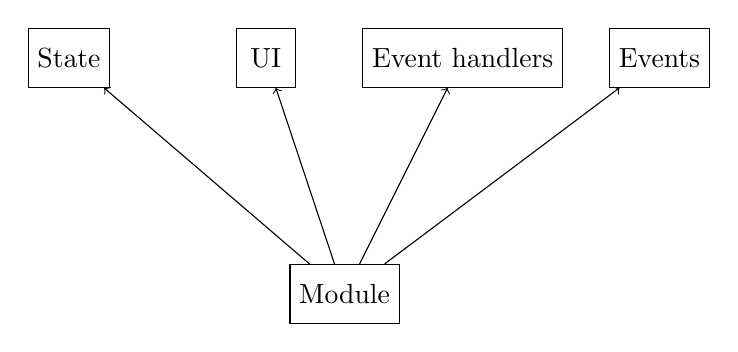
\begin{tikzpicture}
  % Nodes
  \node (state) [rectangle, draw, minimum height=0.75cm, minimum width=1cm] at (-3.5, 0) {State};
  \node (ui) [rectangle, draw, minimum height=0.75cm, minimum width=0.75cm] at (-1, 0) {UI};
  \node (eventH) [rectangle, draw, minimum height=0.75cm, minimum width=0.75cm] at (1.5, 0) {Event handlers};
  \node (event) [rectangle, draw, minimum height=0.75cm, minimum width=0.75cm] at (4, 0) {Events};
  \node (module) [rectangle, draw, minimum height=0.75cm, minimum width=0.75cm] at (0, -3) {Module};
  % Arrow
  \draw[->] (module) to[] node[midway, above] {} (ui);
  \draw[->] (module) to[] node[midway, above] {} (state);
  \draw[->] (module) to[] node[midway, above] {} (event);
  \draw[->] (module) to[] node[midway, above] {} (eventH);
  %\draw[->] (p) to[out=60, in=120] node[midway, above] {Html/State} (i);
  %\draw[->] (i) to[out=-120, in=-60] node[midway, above] {Msg/State} (p);
  % Header
\end{tikzpicture}

    \caption{Initialization stage}
  \end{figure}
\end{frame}


\begin{frame}
  \frametitle{Module Architecture}
  \begin{figure}
    \centering
    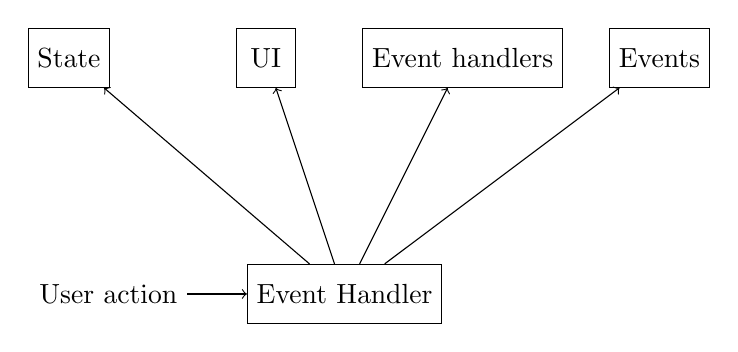
\begin{tikzpicture}
  % Nodes
  \node (state) [rectangle, draw, minimum height=0.75cm, minimum width=1cm] at (-3.5, 0) {State};
  \node (ui) [rectangle, draw, minimum height=0.75cm, minimum width=0.75cm] at (-1, 0) {UI};
  \node (eventH) [rectangle, draw, minimum height=0.75cm, minimum width=0.75cm] at (1.5, 0) {Event handlers};
  \node (event) [rectangle, draw, minimum height=0.75cm, minimum width=0.75cm] at (4, 0) {Events};
  \node (module) [rectangle, draw, minimum height=0.75cm, minimum width=0.75cm] at (0, -3) {Event Handler};
  \node (event0) [] at (-3, -3) {User action};
  % Arrow
  \draw[->] (module) to[] node[midway, above] {} (ui);
  \draw[->] (module) to[] node[midway, above] {} (state);
  \draw[->] (module) to[] node[midway, above] {} (event);
  \draw[->] (module) to[] node[midway, above] {} (eventH);
  \draw[->] (event0) to[] node[midway, above] {} (module);
  %\draw[->] (p) to[out=60, in=120] node[midway, above] {Html/State} (i);
  %\draw[->] (i) to[out=-120, in=-60] node[midway, above] {Msg/State} (p);
  % Header
\end{tikzpicture}

    \caption{Post initialization stage}
  \end{figure}
\end{frame}

\showlogo

\section{Implementation struggles}
\SectionPage

\begin{frame}
  \frametitle{I need super computer time for my featureless app}
  \begin{itemize}
    \item When implementing a prototype
    \pause
    \item \textit{Basic} module, which should only display "Hello, World!"
    \pause
      \begin{figure}
        \centering
        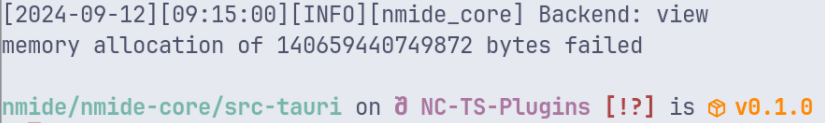
\includegraphics[width=0.9\textwidth]{./pics/memory-allocation-zoomed.png}
        \caption{140.6594 Terabytes of memory}
      \end{figure}
  \end{itemize}
\end{frame}
